\section{Introduction and Goals}

%% figure source is in https://www.dropbox.com/s/slcj04cf0svkkyc/dex1-lsst-mpc-workflows.pptx?dl=0
\begin{figure*}
	\centering
	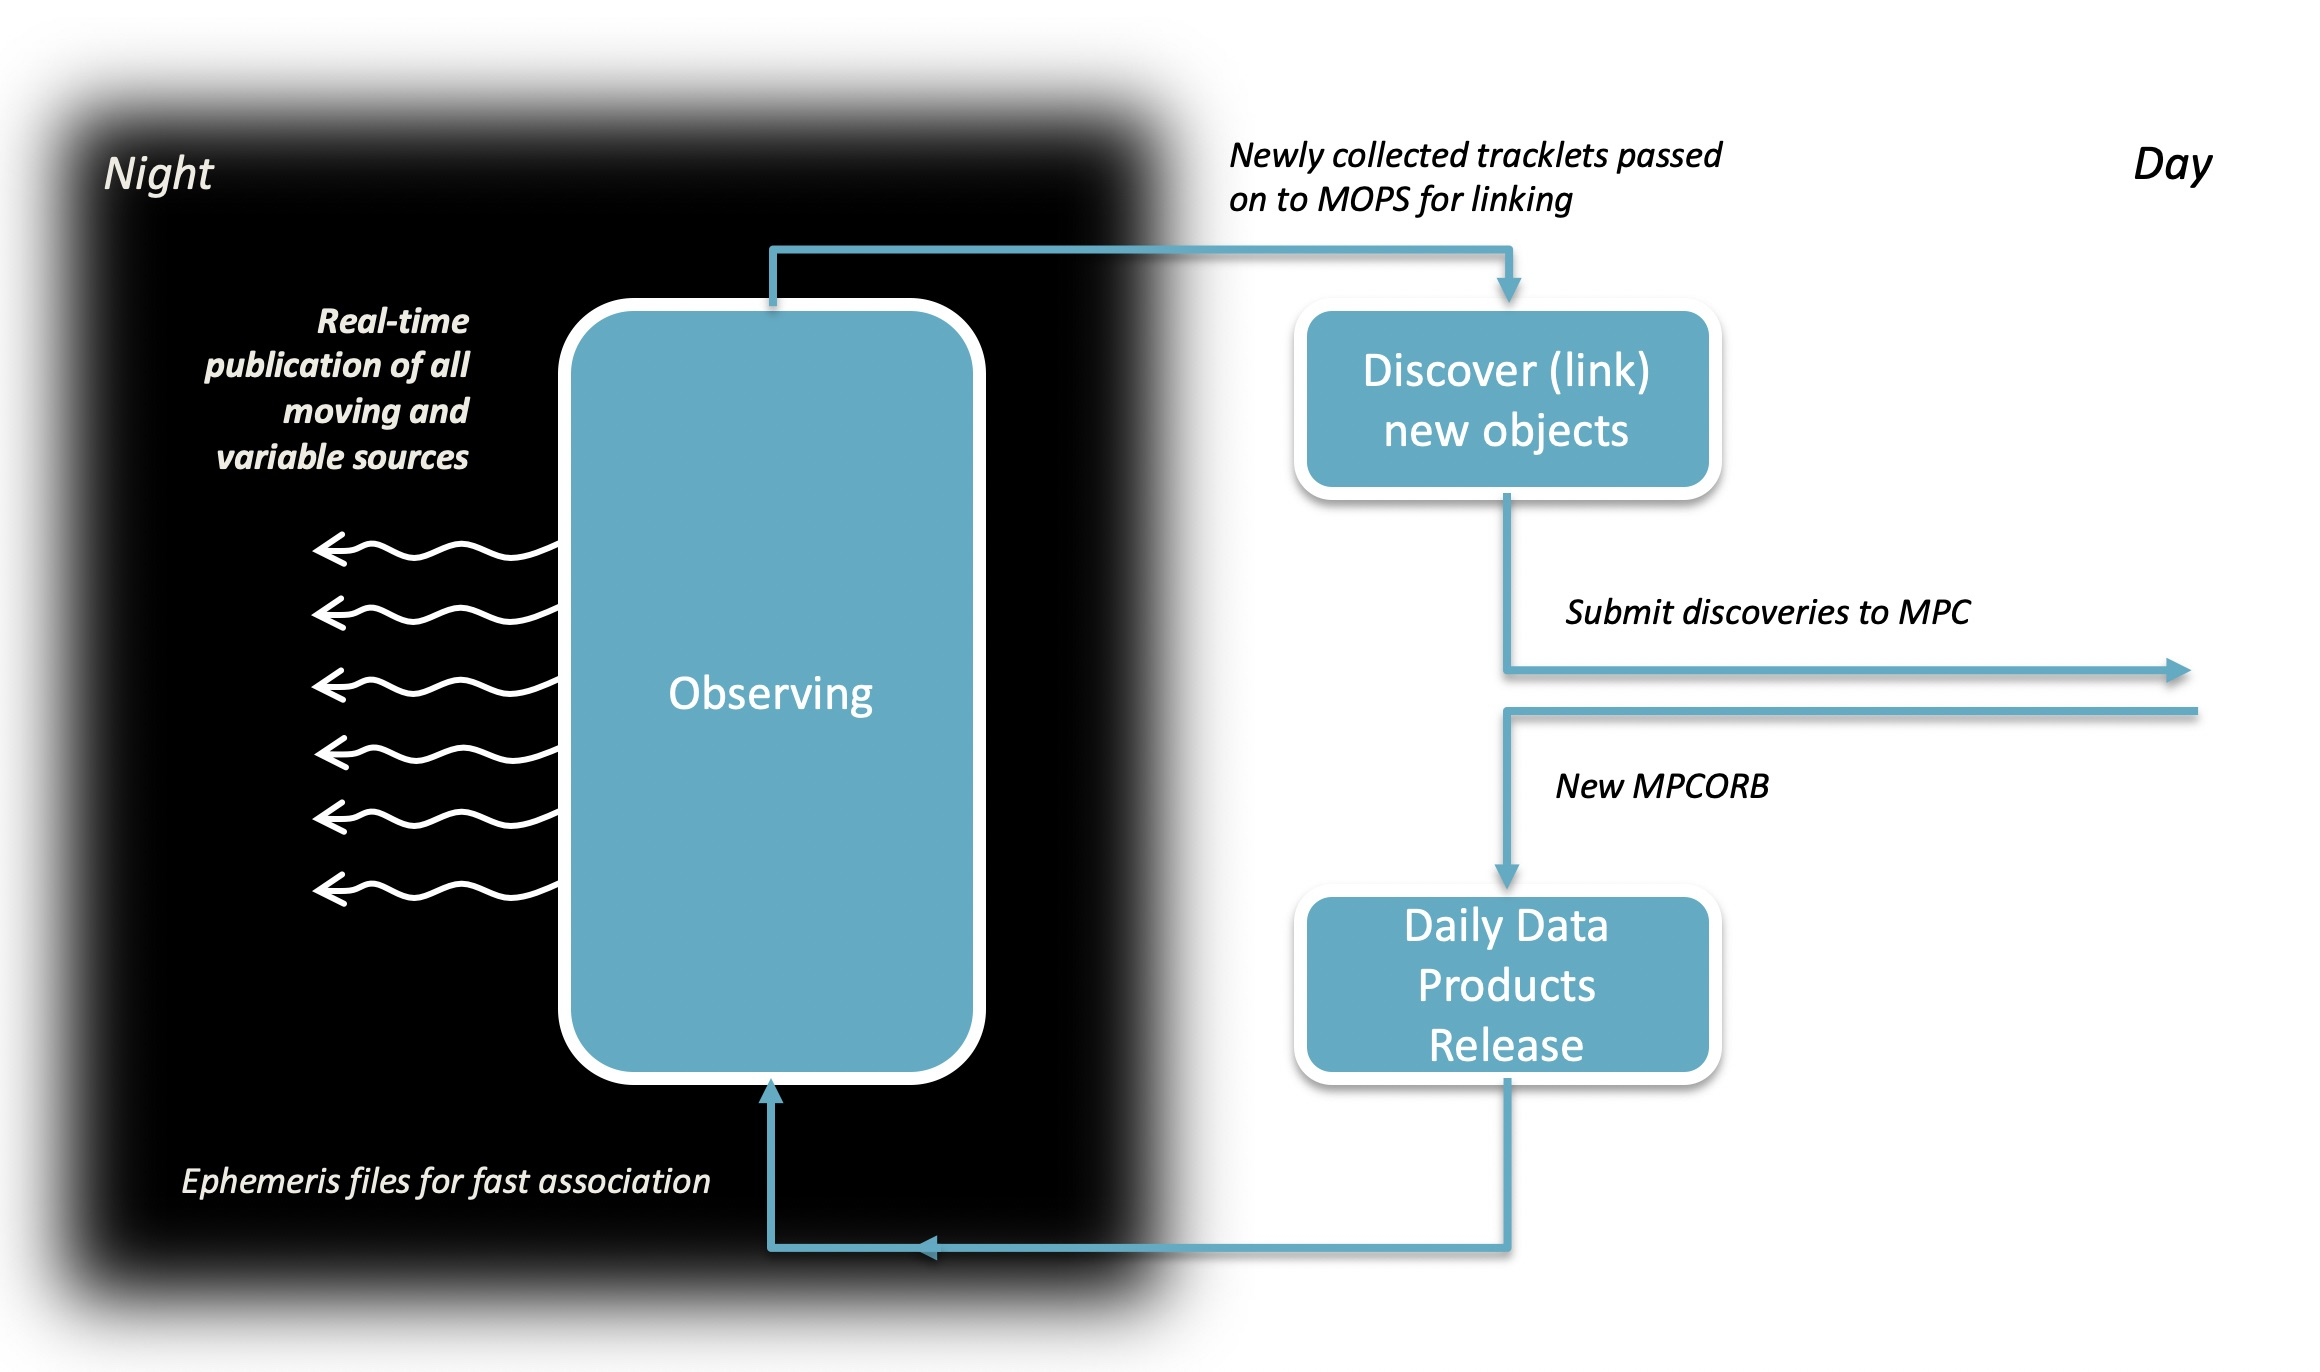
\includegraphics[width=0.9\textwidth]{mpc-loop.jpg}
	\caption{A diagram illustrating the LSST-MPC 24-hr processing loop. The nominal time budgeted for MPC's processing of new data is 4 hours. Consult \url{http://ls.st/ldm-151} for a more detailed breakdown and discussion of individual components.}
	\label{fig:loop}
\end{figure*}

Over its 10-yr program, the Rubin Observatory's Legacy Survey of Space and Time (LSST) is expected to discover over 6 million asteroids, with over 500,000 individual detections and measurements taken and processed, in real time, every night. Rubin's goal is to make these observations and discoveries of Solar System objects available to the scientific community with minimum latency and in a maximally useful fashion. This will be accomplished by promptly submitting them to the MPC after successful linking and/or attribution.

To assure readiness of both Rubin Observatory and the Minor Planet Center to exchange data (see Figure~\ref{fig:loop} for a simplified diagram), we agreed to conduct a series of increasingly complex tests culminating in a full operations-like dress rehearsal sometime in LSST commissioning (not earlier than 2022). This is a brief report summarizing the outcome of the "Data Exchange Text No.1" (DEx1).

\subsection{DEx1 Goals Summary and Objectives}

The main goal of DEx1 was to simulate a dataset expected from the first 2-4 weeks of LSST operations, and exercise the process of sending those data to the MPC, and them being processed by the MPC (to fit orbits to new objects and extend arcs of previously known ones).

The specific objectives of this test were to:
\begin{enumerate}
	\item Assess Rubin's ability to generate valid ADES-formatted submissions.
	\item Assess MPC’s current and expected future ability to ingest LSST-sized submissions.
	\item Exercise/understand the submission process.
	\item Establish relationships with the MPC team.
\end{enumerate}

with one defined stretch goal:
\begin{enumerate}
	\item Test the capability to re-fit orbits and generate a new orbit catalog
\end{enumerate}
\newpage

%We will use the simulated dataset we previously created, but add all the known MPCORB objects into it as well. This has been requested by the MPC, so they can test refits of orbits for known objects.

\section{Test Infrastructure, Software and Environment}
\label{sec:setup}

\noindent {\bf Datasets}: We simulated the first 17 nights of a recently proposed LSST campaign, namely \href{http://astro-lsst-01.astro.washington.edu:8081/allMetricResults?runId=13}{baseline\_2snaps\_v1.5\_10yrs}. The aforementioned OpSim database served as input to a modified version of the \href{https://github.com/AsteroidSurveySimulator/objectsInField}{objectsInField} survey simulator which includes the actual LSST footprint, realistic astrometric ($1\sigma=50$mas) and photometric uncertainties as well as realistic colors for simulated Solar System objects.

The simulated Solar System catalog was comprised of known objects extracted from a current version of the MPCORB catalog (as of September 9, 2020) and supplemented with a faint population ($H>15$mag) drawn from the Synthetic Solar System Model \citep[S3M,][]{2011PASP..123..423G}. Density plots of semimajor axis vs. eccentricity of the simulated populations are shown in Figure \ref{fig:ssodataset}.

Of the simulated Solar System Objects, 888,474 unique objects were observed resulting in 6,931,558 observations over 17 nights (Figure \ref{fig:observations}. The majority of the observed objects were main-belt asteroids (MBAs) with 6,336,214 observations, followed by roughly 20,000 Jupiter Trojans with 52,232 observations and 2645 near-Earth objects (NEOs) with 16,193 observations.
\\

% \note{Siegfried:} briefly describe the simulated dataset -- which populations were used, which OpSim run was used, how it was melded with MPCORB, which MPCORB was used (the date), what was simulated (astrometry + errors), basic dataset stats (e.g., number of objects, observations), etc.

% \begin{table}[]
%     \centering

%     \caption{Caption}
%     \label{tab:my_label}
% \end{table}
\begin{figure}
	\centering
	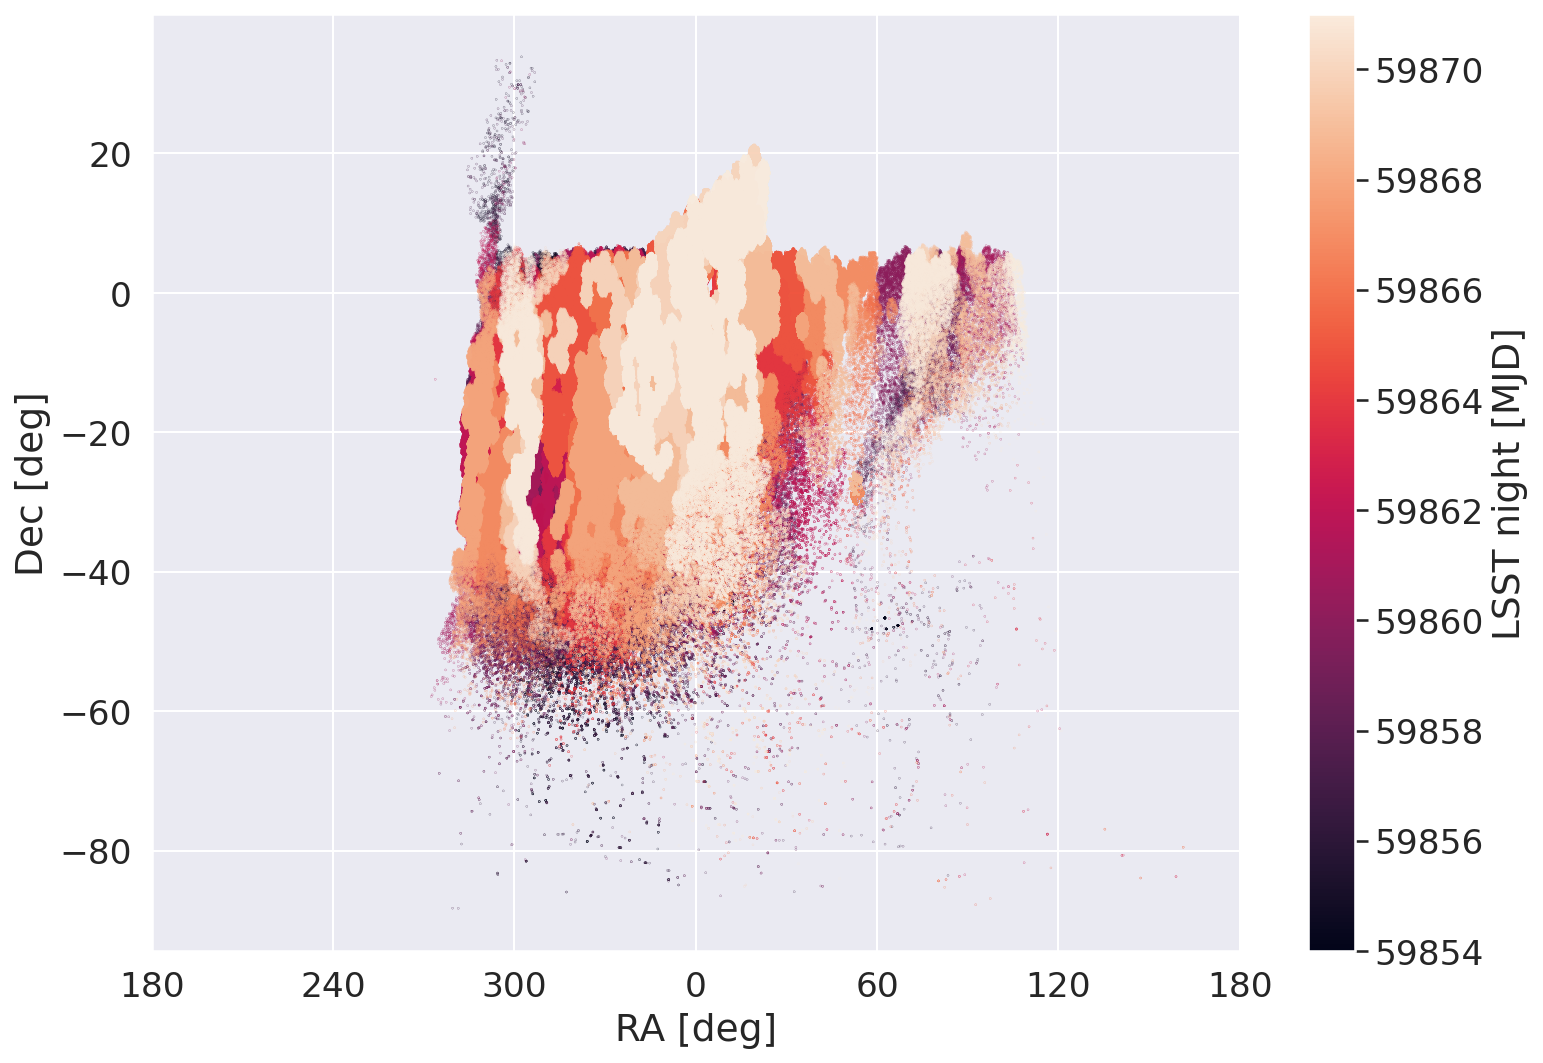
\includegraphics[width=0.9\columnwidth]{observations_n1-17.png}
	\caption{Simulated SSO observations during the first 17 nights of OpSim \href{http://astro-lsst-01.astro.washington.edu:8081/allMetricResults?runId=13}{baseline\_2snaps\_v1.5\_10yrs}.}
	\label{fig:observations}
\end{figure}

\begin{figure}
	\centering
	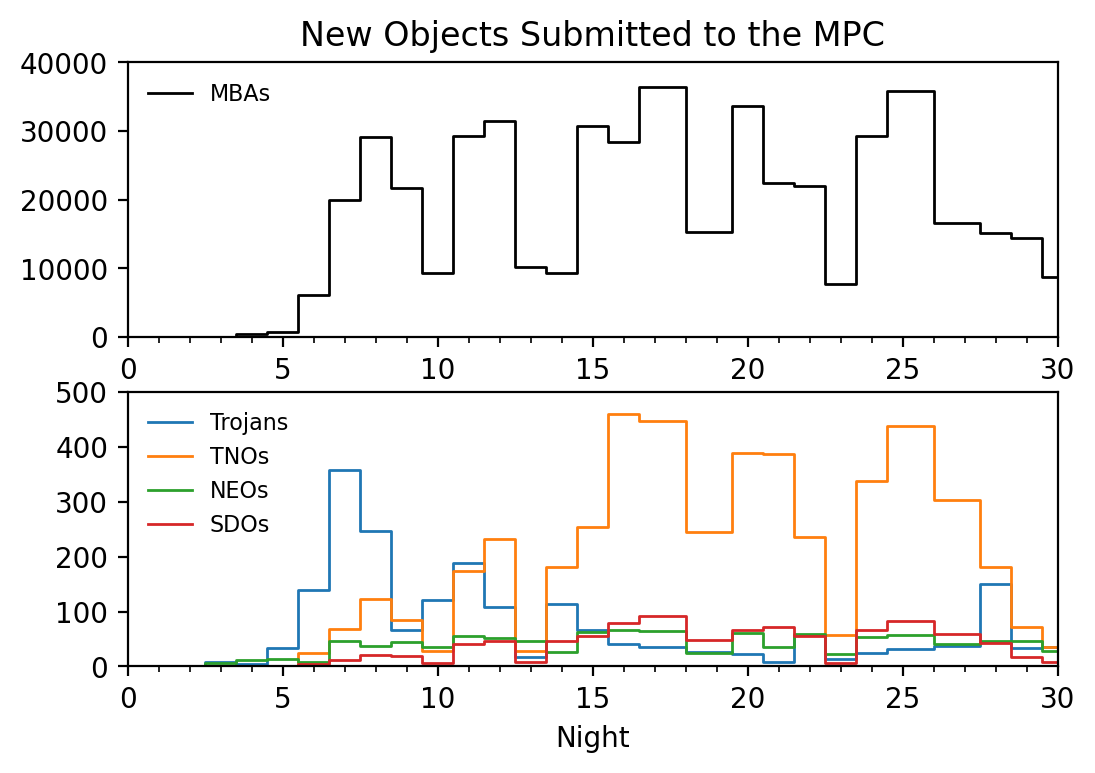
\includegraphics[width=0.9\columnwidth]{discovery_rates.png}
	\caption{A figure showing the number of (mock) newly discovered objects in the first month of a simulated LSST survey. No objects are discovered in the first few nights, as a consequence of LSST's linking algorithm requiring at least three nights of data for identification of a reliable candidate. The subsequent modulation of the discovery rate is due to variations in the coverage of the ecliptic on any given night.}
	\label{fig:lsst_submissions}
\end{figure}

\begin{figure*}
	\centering
	\begin{tabular}{cc}
		NEO & MBA\\
		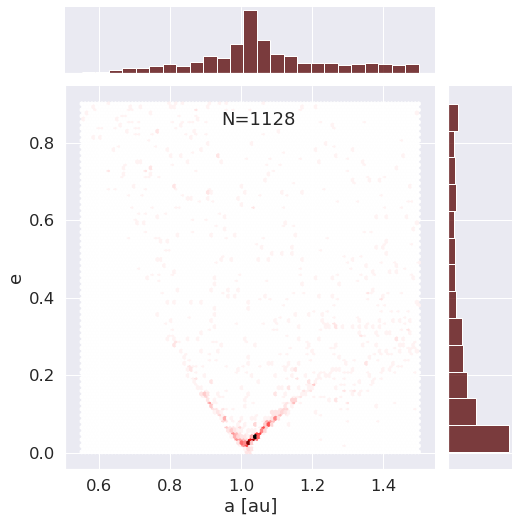
\includegraphics[width=0.5\textwidth]{neo_ae.png} &
		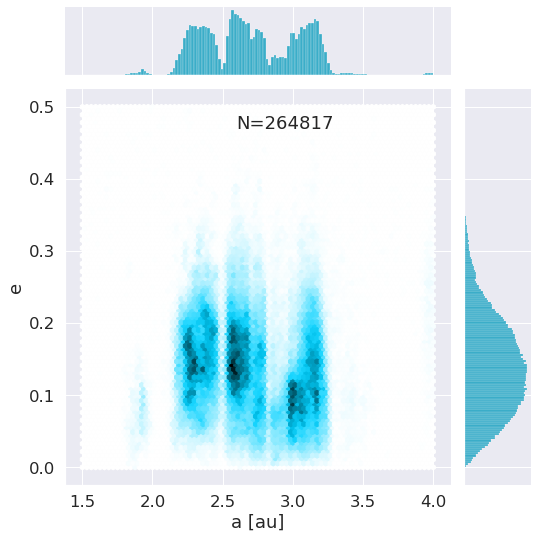
\includegraphics[width=0.5\textwidth]{mba_ae.png} \\
		Jupiter Trojans & TNOs\\
		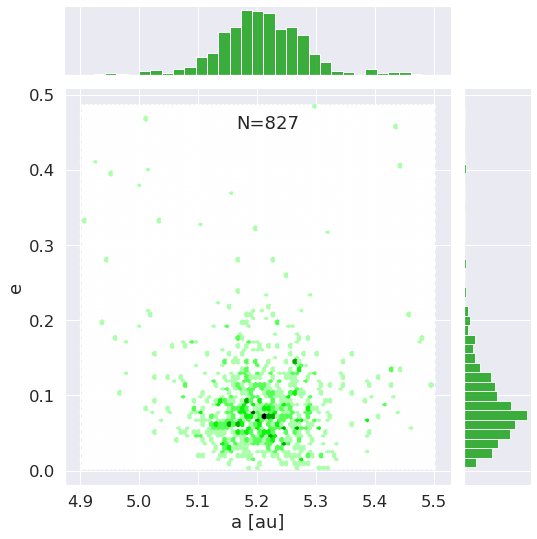
\includegraphics[width=0.5\textwidth]{trojan_ae.png} &
		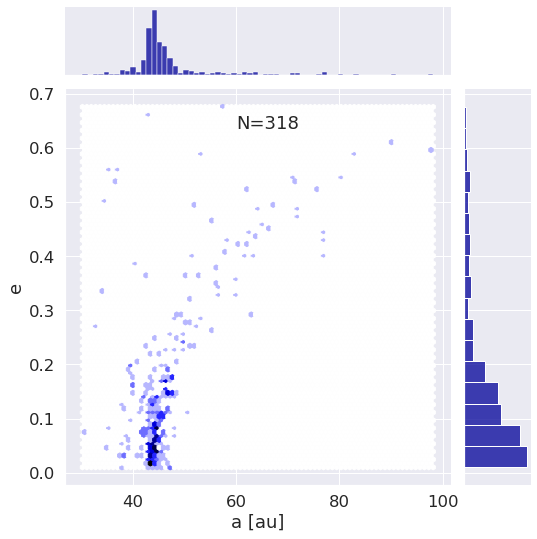
\includegraphics[width=0.5\textwidth]{tno_ae.png}
	\end{tabular}
	
	\caption{Semimajor axis vs orbital eccentricity for known and newly discovered Solar System objects after 17 nights of simulated LSST observations. The number N displayed in the graphs represent the number of objects falling into the plot domain. Those numbers are proxies for the actual number of discoveries.}
	\label{fig:ssodataset}
\end{figure*}

\noindent {\bf Software (LSST)}: We have used the development versions of LSST Solar System Processing Pipelines, part of the broader LSST Data Management suite. These were run on local machines at the University of Washington.
\\

%\noindent {\bf Software (LSST)}: \note{Joachim:} list which LSST/SSP codes were used (difi, attribution?). List relevant github repos. Briefly discuss how diffi was used to generate mock discovery list and re-observed object lists.


\noindent {\bf Software (MPC)}: MPC is currently using a new version of the OrbFit code\footnote{http://adams.dm.unipi.it/orbfit/}, which is not public yet. In particular, the software used for the computation of the orbit of the new object candidates is a new code developed in the last months at the MPC, that will be used for the NEOCP in the near future. The code is still undergoing a testing phase, but it's performing quite well and it's very close to be the code will be permanently used for the short-arc orbit determination, e.g. new objects. 
\\

\noindent {\bf Infrastructure (MPC)}: Two distinct PostgreSQL version 12 database environments were used. The first was a replica of the MPC’s current development database of archived submissions, ~180 million observations, simulating database state at scale during import/load. The second was an Amazon Web Services {\tt r5a.2xlarge} EC2 instance (8 processors, 64GB RAM) with the same schema but no prior data, used to simulate the MPC side of the overall process (import/load, identify known/extend new, orbit update), accessible by both teams.
\\

\noindent {\bf Processes:} Most steps in the tested workflow were executed manually. The objective of this challenge was to ensure that the core data exchange workflow steps and associated data interfaces are understood, and testing automation would add complexity and distract from that objective. Tests of automation will be a subject of future challenges.

\section{Test 1: 21-day dataset}

\subsection{Test description and objectives}

%% figure source is in https://www.dropbox.com/s/slcj04cf0svkkyc/dex1-lsst-mpc-workflows.pptx?dl=0
\begin{figure}
	\centering
	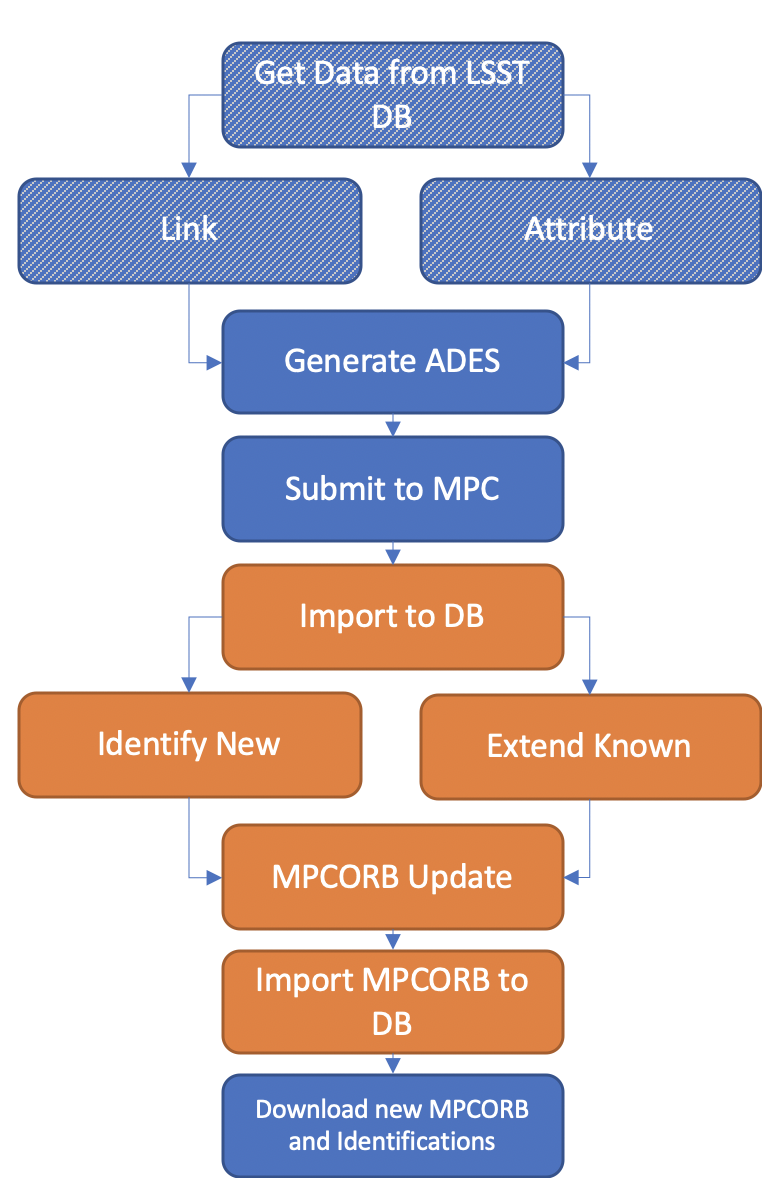
\includegraphics[width=0.9\columnwidth]{test1-workflow.png}
	\caption{Workflow for Test 1. Solid-colored elements used existing prototypes of software or infrastructure, while hatched elements used simulated stand-ins.}
	\label{fig:test1}
\end{figure}

This test consisted of generating ADES files for the first 20 days of the simulated survey, making a submission, and having the MPC process the submission to generate new object identifications and updates to orbits of already known objects.

The test workflow is illustrated in Figure~\ref{fig:test1}. The object identifications were tested for correctness, but not used beyond that (i.e., to attribute objects in the next night of observations).

\subsection{Generated dataset}

% \note{Joachim:}  We generated a series of 21 ADES from the simulated dataset discussed in \ref{sec:setup}... Discuss how they were generated, point to the relevant notebooks on github or give examples of the command line arguments to use to generate them. Add table with the number of objects (known/unknown) for each night, number of observation, and file size for each file. Also add a plot. Add anything you'd like to know yourself when you read this a year from now.

We generated a series of 21 ADES from the simulated dataset discussed in section \ref{sec:setup}. These contained mock observations of already known objects (from the MPCORB part of the simulated catalog), as well as new objects expected to be discovered by LSST's tracklet linking algorithm (Figure~\ref{fig:lsst_submissions}).

\subsection{Test execution}

The {\tt curl} interface for PSV-ADES submission was tested and assured to work, but the bulk of the generated files were delivered to the Minor Planet Center via direct download (for simplicity). There, they were converted to XML-serializes ADES, and ingested into the mock MPC database, simulating the ingestion procedure which will occur in operations. The reported objects were divided into two subsets: new object candidates and observations of known objects, and processed separately. The new object candidates were divide into seven different batches. The new object candidates were verified and their orbits computed using OrbFit. The benchmarks of OrbFit runs are listed in Table~\ref{tab:orbfit_new_objects}. The table contains the total number of objects in each batch, the total number of observations in each batch, the execution time and the failed cases. Those failures correspond to cases for which the whole orbit determination process failed.

\begin{table}[h]
	\resizebox{\columnwidth}{!}{\begin{tabular}{r|r|r|r}
			\hline
			\# of objects & \# of observations & Execution time &   \# of failures\\
			\hline
			30308 & 455050 & 129m 11s & 75\\
			30308 & 455028 & 132m 13s & 78\\
			30308 & 401964 & 142m 15s & 124\\
			30308 & 421253 & 138m 23s & 108\\
			30308 & 434351 & 135m 13s & 98\\
			30308 & 413372 & 139m 10s & 112\\ 
			30307 & 368947 & 125m 11s &136\\
			\hline
	\end{tabular}}
	\caption{Benchmarks of OrbFit runs for new object candidates. The columns contain the total number of processed objects, the total number of observations corresponding to the processed batch, the execution time and the total number of objects for which the orbit determination failed.}
	\label{tab:orbfit_new_objects}
\end{table}

The observations of known objects have been used to extend their arcs and re-fit the orbits, also using orbfit. The time to execute this element was similar to the time to run orbfit on new orbits. The resulting associations and orbits were formatted in MPCORB format, and uploaded to the database. From there, they were queried by the LSST team.

\subsection{Test results}

This test was successful in full. All generated files were successfully submitted to the MPC and individually run through the workflow shown in Figure~\ref{fig:test1}.

Work on attempting to reach the stretch goal and ``close the loop'' continues and will likely form a part of the Data Exchange Test 2.

%The computation for a typical night took XXX on YYY cores, which is alreadu close to the notional 4h processing budget.
%... should we discuss what we learned about rejections, flags? ...
%... what's missing that should be here ...?

%% \section{Test 2: Closing the loop}
%% Tracklets for the first 16 nights of the simulated LSST observations were successfully submitted to the MPC in ADES format. The MPC performed initial orbit determination (IOD) and   
%% \lsst{Siegfried -- could you draft this section and subsections, with style similar to the previous one? Make sure to %% mention this also tests the attribution code. Discuss how we inadvertently tested what would happen after a two week outage (because the file was large)}.
%% 
%% %% figure source is in https://www.dropbox.com/s/slcj04cf0svkkyc/dex1-lsst-mpc-workflows.pptx?dl=0
%% \begin{figure}
%%     \centering
%%     \includegraphics[width=0.9\columnwidth]{test2-workflow.png}
%%     \caption{Workflow for Test 2. Solid-colored elements used existing prototypes of software or infrastructure, while hatched elements used simulated stand-ins.}
%%     \label{fig:test1}
%% \end{figure}
%% 
%% \subsection{Test objectives}
%% 
%% \subsection{Generated dataset}
%% 
%% \subsection{Test results}


\section{Discussion and Key Conclusions}

Key findings and recommendations:
\begin{itemize}
	\item All planned tests were attempted and -- after fixing a few minor uncovered issues -- ultimately successful. Stretch goals were partially executed, with full completion left for a subsequent exercise.
	\item The MPC is likely to be computationally capable to ingest LSST-sized datasets in the first months of LSST, assuming error-free operation. Available MPC computational capacity is already close to what's necessary to turn around the LSST submissions within the notional 4hr budget. No fundamental issues or bottlenecks were identified; assuming the necessary workflow control software is implemented, scaling to required capacity is likely to be a simple matter of adding more cores.
	\item The MPC should ideally plan for the ability to burst computational capacity on order of 10x relative to what it has presently available. This would enable comfortable data processing margins, as well as the ability to deal with unexpectedly large submissions (e.g., such catch-up submission after a multi-day outage). We note that this capacity is not required 24/7, but just over the few hour period when LSST data are being processed. Elastic cloud resources may be an ideal and cost-effective way to acquire it.
	\item Assuming it is fully operational since day one, the LSST is expected to discover approximately 0.5M new objects in the first month of operations. Designating those objects as they're discovered will result in designations with unprecedentedly high cycle counts (e.g., 2023 UX$_{5678}$), which cannot be written in packed form following the present scheme\footnote{The present packing scheme allows for cycle counts up to 629, for only 16,354 discoveries in any half-month -- \url{https://www.minorplanetcenter.net/iau/info/PackedDes.html}}. The packed provisional designation scheme will have to be updated to accommodate (ideally) $O(1\mathrm{M})$ new discoveries in any half-month. Any changes should probably be rolled out soon, to give the community enough time to adapt existing tools that rely on the current format.
	\item Present ADES format specification does not allow a globally unique observation identifier -- {\tt obsId} -- to be generated and submitted for unlinked detections by the observer\footnote{See Note 1 on Page 10 of \url{https://minorplanetcenter.net//iau/info/IAU2015_ADES.pdf}}. Instead, the {\tt obsId} field is assigned by the MPC, and is to be communicated by the observer in an unspecified manner. This creates practical difficulties for the observer in matching the MPC-assigned IDs with any IDs present in their database (especially when the submitted ADES files are automatically generated and considered ephemeral). We propose the ADES specification is updated to allow the {\tt obsId} field to be generated by the observer (following a certain set of rules to ensure global uniqueness), rather than the MPC. Alternatively, another observer-specified ID field -- e.g., {\tt localObsId} -- could be added. This change would make the MPC database system as well as the observer's databases significantly less complex and more robust.
	\item The LSST should develop a realistic hybrid MPCORB+simulated populations catalog for future experiments. The simple $H > 15$ cut used to construct the merged catalog in this set of experiments inadvertantly excluded all simulated KBOs from the datasets.
	\item The ability to obtain data by directly querying the MPC database has been tremendously useful. While this introduces a tight coupling with the database schema (i.e., any change in the database schema may break the code that depends on it), the accelerated development enabled by it may make it a worthwhile tradeoff.
	\item The MPC and Rubin teams worked well together, with no collaboration issues. Having staff with small bodies expertise on the Rubin team enabled a quick ``impedance match'' to be established between the teams. Ability to directly message via a dedicated Slack channel has proven immensely useful. While originally planned to be done in-person, the entire data exchange challenge was conducted remotely.
\end{itemize}

Caveats and future work:
\begin{itemize}
	\item This test did not address operations in more realistic conditions, such as having erroneous associations or other mistakes that may require manual intervention. Those will be addressed in a future challenge.
	\item Future tests will focus on automating most elements of the data exchange workflow, and testing of automated data exchange interfaces and processes. The verification of automation and the ability to scale is likely to be our next challenge.
	\item We have not tested resubmissions of large amounts of data, such as those which will be occurring after annual LSST data releases when improved astrometry and photometry become available. This is left for future tests.
\end{itemize}

\acknowledgements

This material is based upon work supported in part by the National Science Foundation through Cooperative Agreement 1258333 managed by the Association of Universities for Research in Astronomy (AURA), and the Department of Energy under Contract No. DEAC02-76SF00515 with the SLAC National Accelerator Laboratory. Additional LSST funding comes from private donations, grants to universities, and in-kind support from LSSTC Institutional Members. MJ and JM wish to acknowledge the support of the Washington Research Foundation Data Science Term Chair fund, and the University of Washington Provost’s Initiative in Data-Intensive Discovery.

\bibliography{local}{}
\bibliographystyle{aasjournal}

%% This command is needed to show the entire author+affiliation list when
%% the collaboration and author truncation commands are used.  It has to
%% go at the end of the manuscript.
%\allauthors

%% Include this line if you are using the \added, \replaced, \deleted
%% commands to see a summary list of all changes at the end of the article.
%\listofchanges

\end{document}

